\documentclass[12pt, titlepage]{article}

\usepackage{fullpage}
\usepackage[round]{natbib}
\usepackage{multirow}
\usepackage{booktabs}
\usepackage{tabularx}
\usepackage{graphicx}
\usepackage{float}
\usepackage{hyperref}
\hypersetup{
    colorlinks,
    citecolor=blue,
    filecolor=black,
    linkcolor=red,
    urlcolor=blue
}
\usepackage{tikz}
\usetikzlibrary{shapes.geometric, arrows}
\usepackage{pdflscape}

\newcommand{\ProjectName}{ESF }

\input{../../Comments}
\input{../../Common}

\newcounter{acnum}
\newcommand{\actheacnum}{AC\theacnum}
\newcommand{\acref}[1]{AC\ref{#1}}

\newcounter{ucnum}
\newcommand{\uctheucnum}{UC\theucnum}
\newcommand{\uref}[1]{UC\ref{#1}}

\newcounter{mnum}
\newcommand{\mthemnum}{M\themnum}
\newcommand{\mref}[1]{M\ref{#1}}

\tikzstyle{process} = [rectangle, minimum width=2cm, text width=2.4cm, minimum height=1cm, text centered, draw=black, fill=gray!30]

\begin{document}

\title{Module Guide for \ProjectName} 
\author{Alaap Grandhi}
\date{\today}

\maketitle

\pagenumbering{roman}

\section{Revision History}

\begin{tabularx}{\textwidth}{p{3cm}p{2cm}X}
\toprule {\bf Date} & {\bf Version} & {\bf Notes}\\
\midrule
Mar 21 & 1.0 & Initial Draft\\
Mar 22 & 1.1 & Added Anticipated and Unlikely Changes\\
Apr 17 & 2.0 & Added Professor Smith's feedback\\
Apr 17 & 2.1 & Added Domain Expert feedback\\
\bottomrule
\end{tabularx}

\newpage

\section{Reference Material}

This section records information for easy reference.

\subsection{Abbreviations and Acronyms}

\renewcommand{\arraystretch}{1.2}
\begin{tabular}{l l} 
  \toprule		
  \textbf{symbol} & \textbf{description}\\
  \midrule 
  AC & Anticipated Change\\
  DAG & Directed Acyclic Graph \\
  M & Module \\
  MG & Module Guide \\
  OS & Operating System \\
  R & Requirement\\
  SC & Scientific Computing \\
  SRS & Software Requirements Specification\\
  \ProjectName & Equivariant Sensor Fusion\\
  UC & Unlikely Change \\
  \bottomrule
\end{tabular}\\

\newpage

\tableofcontents

\listoftables

\listoffigures

\newpage

\pagenumbering{arabic}

\section{Introduction}

Decomposing a system into modules is a commonly accepted approach to developing
software.  A module is a work assignment for a programmer or programming
team~\citep{ParnasEtAl1984}.  We advocate a decomposition
based on the principle of information hiding~\citep{Parnas1972a}.  This
principle supports design for change, because the ``secrets'' that each module
hides represent likely future changes.  Design for change is valuable in SC,
where modifications are frequent, especially during initial development as the
solution space is explored.  

Our design follows the rules layed out by \citet{ParnasEtAl1984}, as follows:
\begin{itemize}
\item System details that are likely to change independently should be the
  secrets of separate modules.
\item Each data structure is implemented in only one module.
\item Any other program that requires information stored in a module's data
  structures must obtain it by calling access programs belonging to that module.
\end{itemize}

After completing the first stage of the design, the Software Requirements
Specification (SRS), the Module Guide (MG) is developed~\citep{ParnasEtAl1984}. The MG
specifies the modular structure of the system and is intended to allow both
designers and maintainers to easily identify the parts of the software.  The
potential readers of this document are as follows:

\begin{itemize}
\item New project members: This document can be a guide for a new project member
  to easily understand the overall structure and quickly find the
  relevant modules they are searching for.
\item Maintainers: The hierarchical structure of the module guide improves the
  maintainers' understanding when they need to make changes to the system. It is
  important for a maintainer to update the relevant sections of the document
  after changes have been made.
\item Designers: Once the module guide has been written, it can be used to
  check for consistency, feasibility, and flexibility. Designers can verify the
  system in various ways, such as consistency among modules, feasibility of the
  decomposition, and flexibility of the design.
\end{itemize}

The rest of the document is organized as follows. Section
\ref{SecChange} lists the anticipated and unlikely changes of the software
requirements. Section \ref{SecMH} summarizes the module decomposition that
was constructed according to the likely changes. Section \ref{SecConnection}
specifies the connections between the software requirements and the
modules. Section \ref{SecMD} gives a detailed description of the
modules. Section \ref{SecTM} includes two traceability matrices. One checks
the completeness of the design against the requirements provided in the SRS. The
other shows the relation between anticipated changes and the modules. Section
\ref{SecUse} describes the use relation between modules.

\section{Anticipated and Unlikely Changes} \label{SecChange}

This section lists possible changes to the system. According to the likeliness
of the change, the possible changes are classified into two
categories. Anticipated changes are listed in Section \ref{SecAchange}, and
unlikely changes are listed in Section \ref{SecUchange}.

\subsection{Anticipated Changes} \label{SecAchange}

Anticipated changes are the source of the information that is to be hidden
inside the modules. Ideally, changing one of the anticipated changes will only
require changing the one module that hides the associated decision. The approach
adapted here is called design for
change.

\begin{description}
\item[\refstepcounter{acnum} \actheacnum \label{acHardware}:] The specific
  hardware on which the software is running.
\item[\refstepcounter{acnum} \actheacnum \label{acInput}:] The format of the
  input images and LiDAR.
\item[\refstepcounter{acnum} \actheacnum \label{acLoss}:] The loss function used for training.
\item[\refstepcounter{acnum} \actheacnum \label{acEQLayers}:] The specific equivariant layer implementation
  used.
\item[\refstepcounter{acnum} \actheacnum \label{acOptim}:] The specific version of ADAM used for optimization.
\item[\refstepcounter{acnum} \actheacnum \label{acData}:] The choice of training datasets (expanding beyond just NuScenes and Waymo).
\item[\refstepcounter{acnum} \actheacnum \label{acMetric}:] The metrics collected for evaluation (adding more than just mAP).
\item[\refstepcounter{acnum} \actheacnum \label{acLogging}:] The choice of library for logging. 
\item[\refstepcounter{acnum} \actheacnum \label{acConfig}:] The configuration file format.
\item[\refstepcounter{acnum} \actheacnum \label{acPlots}:] The choice of library for generating 3D visualizations of predicted bounding boxes.    
\end{description}

\subsection{Unlikely Changes} \label{SecUchange}

The module design should be as general as possible. However, a general system is
more complex. Sometimes this complexity is not necessary. Fixing some design
decisions at the system architecture stage can simplify the software design. If
these decision should later need to be changed, then many parts of the design
will potentially need to be modified. Hence, it is not intended that these
decisions will be changed.

\begin{description}
\item[\refstepcounter{ucnum} \uctheucnum \label{ucPyTorch}:] The use of PyTorch in the construction of many of the modules.
\item[\refstepcounter{ucnum} \uctheucnum \label{ucDL}:] The use of a deep-learning based model.
\item[\refstepcounter{ucnum} \uctheucnum \label{ucSL}:] The use of supervised learning techniques to train the model. 
\item[\refstepcounter{ucnum} \uctheucnum \label{ucOpenPCDet}:] The use of OpenPCDet as a foundation for the code.
\end{description}

\section{Module Hierarchy} \label{SecMH}

This section provides an overview of the module design. Modules are summarized
in a hierarchy decomposed by secrets in Table \ref{TblMH}. The modules listed
below, which are leaves in the hierarchy tree, are the modules that will
actually be implemented.

\begin{description}
\item [\refstepcounter{mnum} \mthemnum \label{mHH}:] Hardware-Hiding Module
\item [\refstepcounter{mnum} \mthemnum \label{mCo}:] Config Module
\item [\refstepcounter{mnum} \mthemnum \label{mD}:] Data Module
\item [\refstepcounter{mnum} \mthemnum \label{mM}:] Model Module
\item [\refstepcounter{mnum} \mthemnum \label{mCh}:] Checkpoint Module
\item [\refstepcounter{mnum} \mthemnum \label{mT}:] Training Module
\item [\refstepcounter{mnum} \mthemnum \label{mI}:] Inference Module
\item [\refstepcounter{mnum} \mthemnum \label{mLo}:] Loss Module
\item [\refstepcounter{mnum} \mthemnum \label{mE}:] Evaluation Module
\item [\refstepcounter{mnum} \mthemnum \label{mO}:] Optimization Module
\item [\refstepcounter{mnum} \mthemnum \label{mDP}:] Data Processing Module
\item [\refstepcounter{mnum} \mthemnum \label{mEL}:] Equivariant Layer Module
\item [\refstepcounter{mnum} \mthemnum \label{mOL}:] OpenPCDet Layer Module
\item [\refstepcounter{mnum} \mthemnum \label{mPl}:] Plotting Module
\item [\refstepcounter{mnum} \mthemnum \label{mPy}:] PyTorch Module
\item [\refstepcounter{mnum} \mthemnum \label{mLg}:] Logging Module
\end{description}


\begin{table}[h!]
\centering
\begin{tabular}{p{0.3\textwidth} p{0.6\textwidth}}
\toprule
\textbf{Level 1} & \textbf{Level 2}\\
\midrule

{Hardware-Hiding Module} & ~ \\
\midrule

\multirow{7}{0.3\textwidth}{Behaviour-Hiding Module} 
& Config Module\\
& Data Module\\
& Model Module\\
& Checkpoint Module\\
& Training Module\\
& Inference Module\\
& Loss Module\\ 
& Evaluation Module\\
& Optimization Module\\
& Data Processing Module\\
& Equivariant Layer Module\\
& OpenPCDet Layer Module\\
\midrule

\multirow{3}{0.3\textwidth}{Software Decision Module}
& Plotting Module\\
& PyTorch Module\\
& Logging Module\\
\bottomrule

\end{tabular}
\caption{Module Hierarchy}
\label{TblMH}
\end{table}

\section{Connection Between Requirements and Design} \label{SecConnection}

The design of the system is intended to satisfy the requirements developed in
the SRS. In this stage, the system is decomposed into modules. The connection
between requirements and modules is listed in Table~\ref{TblRT}.

\section{Module Decomposition} \label{SecMD}

Modules are decomposed according to the principle of ``information hiding''
proposed by \citet{ParnasEtAl1984}. The \emph{Secrets} field in a module
decomposition is a brief statement of the design decision hidden by the
module. The \emph{Services} field specifies \emph{what} the module will do
without documenting \emph{how} to do it. For each module, a suggestion for the
implementing software is given under the \emph{Implemented By} title. If the
entry is \emph{OS}, this means that the module is provided by the operating
system or by standard programming language libraries.  \emph{\progname{}} means the
module will be implemented by the \progname{} software.

Only the leaf modules in the hierarchy have to be implemented. If a dash
(\emph{--}) is shown, this means that the module is not a leaf and will not have
to be implemented.

\subsection{Hardware Hiding Modules (\mref{mHH})}

\begin{description}
\item[Secrets:]The data structure and algorithm used to implement the virtual
  hardware.
\item[Services:]Serves as a virtual hardware used by the rest of the
  system. This module provides the interface between the hardware and the
  software. So, the system can use it to display outputs or to accept inputs.
\item[Implemented By:] OS
\end{description}

\subsection{Behaviour-Hiding Modules}

\begin{description}
\item[Secrets:]The contents of the required behaviours.
\item[Services:]Includes programs that provide externally visible behaviour of
  the system as specified in the software requirements specification (SRS)
  documents. This module serves as a communication layer between the
  hardware-hiding module and the software decision module. The programs in this
  module will need to change if there are changes in the SRS.
\item[Implemented By:] --
\end{description}

[Record, Library, Abstract Object, or Abstract Data Type]

\subsubsection{Config Module (\mref{mCo})}
\begin{description}
\item[Secrets:] The format and structure of the input configuration.
\item[Services:] Loads the configuration from a predefined file and makes it accessible to other modules.
\item[Implemented By:] \ProjectName{} 
\item[Type of Module:] Abstract Object
\end{description}

\subsubsection{Data Module (\mref{mD})}
\begin{description}
\item[Secrets:] The format and structure of the training and evaluation datasets along with their respective loaders.
\item[Services:] Loads the input data and packages it in a form (a dataloader) that facilitates batched training.
\item[Implemented By:] \ProjectName{}
\item[Type of Module:] Abstract Data Type
\end{description}

\subsubsection{Model Module (\mref{mM})}
\begin{description}
\item[Secrets:] The format and structure of the deep learning fusion model.
\item[Services:] Forms a learnable and differentiable mapping from input images and LiDAR to predicted bounding boxes.
\item[Implemented By:] \ProjectName{}
\item[Type of Module:] Abstract Data Type
\end{description}
\subsubsection{Etc.}

\subsubsection{Checkpoint Module (\mref{mCh})}
\begin{description}
\item[Secrets:] The methods for saving and loading a model from the file system..
\item[Services:] Allows for the saving of trained models to the file system and the loading of model weights from the file system.
\item[Implemented By:] \ProjectName{}
\item[Type of Module:] Library
\end{description}

\subsubsection{Training Module (\mref{mT})}
\begin{description}
\item[Secrets:] The process by which a model is trained on the input dataset.
\item[Services:] Trains the model on the input dataset using the loss function and the optimizer specified in the configuration file.
\item[Implemented By:] \ProjectName{}
\item[Type of Module:] Library
\end{description}
\subsection{Software Decision Module}

\subsubsection{Inference Module (\mref{mI})}
\begin{description}
\item[Secrets:] The process by which a model is run in inference on some input scene.
\item[Services:] Uses a trained model to produce a visualization of predicted bounding boxes on an input scene.
\item[Implemented By:] \ProjectName{}
\item[Type of Module:] Library
\end{description}

\subsubsection{Loss Module (\mref{mLo})}
\begin{description}
\item[Secrets:] The method by which a loss value is produced from a given input.
\item[Services:] Compares a model's predicted bounding boxes to the ground truth bounding boxes for a given scene in order to produce a loss value.
\item[Implemented By:] \ProjectName{}
\item[Type of Module:] Abstract Data Type
\end{description}

\subsubsection{Evaluation Module (\mref{mE})}
\begin{description}
\item[Secrets:] The method by which a model is evaluated. 
\item[Services:] Compares a model's predicted bounding boxes to the ground truth bounding boxes on some evaluation set to produce an mAP metric for the model.
\item[Implemented By:] \ProjectName{}
\item[Type of Module:] Library
\end{description}

\subsubsection{Optimization Module (\mref{mO})}
\begin{description}
\item[Secrets:] The method by which a model's parameters are updated.
\item[Services:] Updates a model's parameters according to the gradients stored on them using the ADAM algorithm. These gradients themselves are generated by the Loss module.
\item[Implemented By:] \ProjectName{}
\item[Type of Module:] Abstract Data Type
\end{description}

\subsubsection{Data Processing Module (\mref{mDP})}
\begin{description}
\item[Secrets:] The method by which input data is converted into a usable format.
\item[Services:] Converts the input images and input LiDAR into a PyTorch Tensor format that can directly be used for training.
\item[Implemented By:] \ProjectName{} 
\item[Type of Module:] Library
\end{description}

\subsubsection{Equivariant Layer Module (\mref{mEL})}
\begin{description}
\item[Secrets:] The format and the structure of the equivariant layers that will be used to enhance fusion object detection performance.
\item[Services:] Creates equivariant layers that can then be put together to comprise the model. 
\item[Implemented By:] \ProjectName{} using escnn (\cite{cesa2022a}) and equivariant transformer (\cite{tai2019equivariant})
\item[Type of Module:] Abstract Data Type
\end{description}

\subsubsection{OpenPCDet Layer Module (\mref{mOL})}
\begin{description}
\item[Secrets:] The format and the structure of the existing OpenPCDet layers.
\item[Services:] Creates layers that can be put together to form the base BEVFusion model and that will be used for parts of the model.
\item[Implemented By:] OpenPCDet (\cite{openpcdet2020})
\item[Type of Module:] Abstract Data Type
\end{description}

\begin{description}
\item[Secrets:] The design decision based on mathematical theorems, physical
  facts, or programming considerations. The secrets of this module are
  \emph{not} described in the SRS.
\item[Services:] Includes data structure and algorithms used in the system that
  do not provide direct interaction with the user. 
\item[Implemented By:] --
\end{description}

\subsubsection{Plotting Module (\mref{mPl})}
\begin{description}
\item[Secrets:] The method by which to generate 3D visualizations of bounding box predictions
\item[Services:] Provides methods which allow for LiDAR pointcloud scenes to be plotted in 3D alongside ground truth and predicted bounding boxes. 
\item[Implemented By:] \ProjectName{} using Open3D
\item[Type of Module:] Library
\end{description}

\subsubsection{PyTorch Module (\mref{mPy})}
\begin{description}
\item[Secrets:] The set of data structures and algorithms contained within the PyTorch library
\item[Services:] Allows for the creation of datasets, dataloaders, and models for the purposes of Deep-Learning training
\item[Implemented By:] PyTorch
\item[Type of Module:] Records, Libraries, Abstract Data Types
\end{description}

\subsubsection{Logging Module (\mref{mLg})}
\begin{description}
\item[Secrets:] The method by which to log statistics about model training and evaluation.
\item[Services:] Logs loss during training and mAP during evaluation to a file where they can be easily visualized later.
\item[Implemented By:] \ProjectName using a wrapper around Tensorboard
\item[Type of Module:] Abstract Object
\end{description}

\section{Traceability Matrix} \label{SecTM}

This section shows two traceability matrices: between the modules and the
requirements and between the modules and the anticipated changes.

% the table should use mref, the requirements should be named, use something
% like fref
\begin{table}[H]
\centering
\begin{tabular}{p{0.2\textwidth} p{0.6\textwidth}}
\toprule
\textbf{Req.} & \textbf{Modules}\\
\midrule
R1 & \mref{mDP}, \mref{mD}\\
R2 & \mref{mDP}, \mref{mD}\\
R3 & \mref{mHH}, \mref{mCo}, \mref{mD}, \mref{mM}, \mref{mCh}, \mref{mT}, \mref{mLo}, \mref{mE}, \mref{mO}, \mref{mDP}, \mref{mEL}, \mref{mOL}, \mref{mPy}, \mref{mLg}\\
R4 & \mref{mHH}, \mref{mCo}, \mref{mM}, \mref{mCh}, \mref{mI}, \mref{mDP}, \mref{mEL}, \mref{mOL}, \mref{mPl}, \mref{mPy}\\
\bottomrule
\end{tabular}
\caption{Trace Between Requirements and Modules}
\label{TblRT}
\end{table}

\begin{table}[H]
\centering
\begin{tabular}{p{0.2\textwidth} p{0.6\textwidth}}
\toprule
\textbf{AC} & \textbf{Modules}\\
\midrule
\acref{acHardware} & \mref{mHH}\\
\acref{acInput} & \mref{mDP}\\
\acref{acLoss} & \mref{mLo}\\
\acref{acEQLayers} & \mref{mEL}\\
\acref{acOptim} & \mref{mO}\\
\acref{acData} & \mref{mD}\\
\acref{acMetric} & \mref{mE}\\
\acref{acLogging} & \mref{mLg}\\
\acref{acConfig} & \mref{mCo}\\
\acref{acPlots} & \mref{mPl}\\
\bottomrule
\end{tabular}
\caption{Trace Between Anticipated Changes and Modules}
\label{TblACT}
\end{table}

\section{Use Hierarchy Between Modules} \label{SecUse}

In this section, the uses hierarchy between modules is
provided. \citet{Parnas1978} said of two programs A and B that A {\em uses} B if
correct execution of B may be necessary for A to complete the task described in
its specification. That is, A {\em uses} B if there exist situations in which
the correct functioning of A depends upon the availability of a correct
implementation of B.  Figure \ref{FigUH} illustrates the use relation between
the modules. It can be seen that the graph is a directed acyclic graph
(DAG). Each level of the hierarchy offers a testable and usable subset of the
system, and modules in the higher level of the hierarchy are essentially simpler
because they use modules from the lower levels.

\newpage
\begin{landscape}
  \begin{figure}
    \centering
    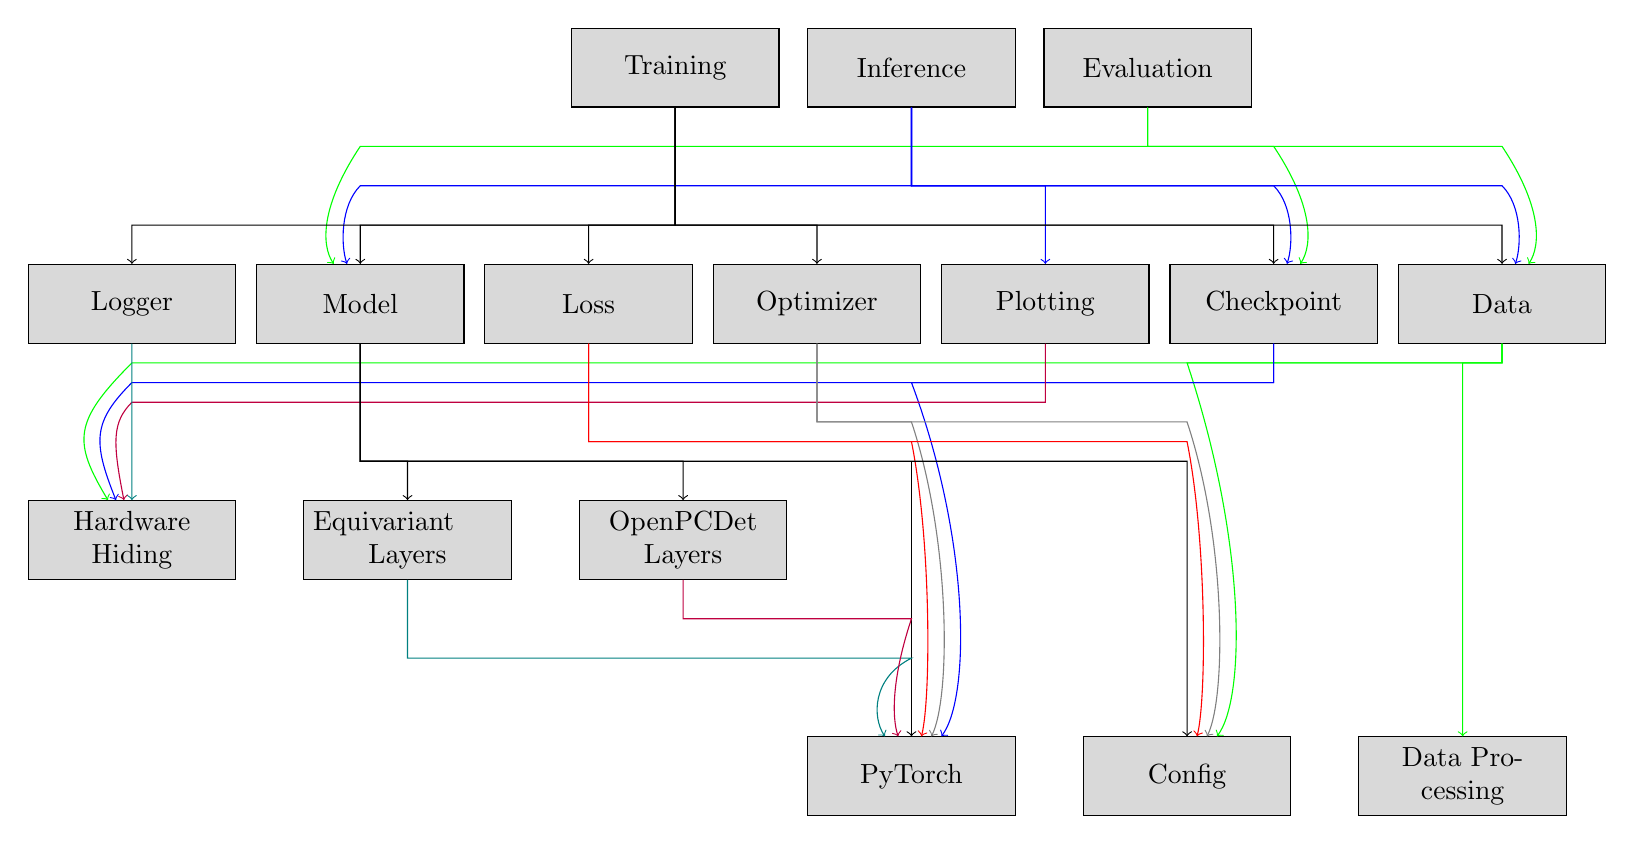
\begin{tikzpicture}[node distance=3cm]
      \node (training) [process] {Training};
      \node (inference) [process, right of=training] {Inference};
      \node (eval) [process, right of=inference] {Evaluation};
      \node (logger) [process, below of=training, xshift=-6.9cm] {Logger};
      \node (model) [process, right of=logger, xshift=-0.1cm] {Model};
      \node (loss) [process, right of=model, xshift=-0.1cm] {Loss};
      \node (optim) [process, right of=loss, xshift=-0.1cm] {Optimizer};
      \node (plot) [process, right of=optim, xshift=-0.1cm] {Plotting};
      \node (ckpt) [process, right of=plot, xshift=-0.1cm] {Checkpoint};
      \node (data) [process, right of=ckpt, xshift=-0.1cm] {Data};
      \node (hardware) [process, below of=logger] {Hardware Hiding};
      \node (eqlayers) [process, right of=hardware, xshift=0.5cm] {Equivariant \newline Layers};
      \node (pcdetlayers) [process, right of=eqlayers, xshift=0.5cm] {OpenPCDet Layers}; 
      \node (torch) [process, below of=pcdetlayers, xshift=2.9cm] {PyTorch};
      \node (config) [process, right of=torch, xshift=0.5cm] {Config};
      \node (dataproc) [process, right of=config, xshift=0.5cm] {Data Processing};
      
      \draw [->, color=green] (eval) |- (7.6, -1) .. controls (8.1, -1.75) and (8.1, -2.25) .. (ckpt);
      \draw [->, color=green] (eval) |- (10.5, -1) .. controls (11, -1.75) and (11, -2.25) .. (data);
      \draw [->, color=green] (eval) |- (-4, -1) .. controls (-4.5, -1.75) and (-4.5, -2.25) .. (model);

      \draw [->, color=blue] (inference) |- (4.7, -1.5) -- (plot);
      \draw [->, color=blue] (inference) |- (7.6, -1.5) .. controls (7.85, -1.75) and (7.85, -2.25) .. (ckpt);
      \draw [->, color=blue] (inference) |- (10.5, -1.5) .. controls (10.75, -1.75) and (10.75, -2.25) .. (data);
      \draw [->, color=blue] (inference) |- (-4, -1.5) .. controls (-4.25, -1.75) and (-4.25, -2.25) .. (model);

      \draw [->] (training) |- (-1.1, -2) -- (loss);
      \draw [->] (training) |- (1.8, -2) -- (optim);
      \draw [->] (training) |- (7.6, -2) -- (ckpt);
      \draw [->] (training) |- (-4, -2) -- (model);
      \draw [->] (training) |- (10.5, -2) -- (data);
      \draw [->] (training) |- (-6.9, -2) -- (logger);

      \draw [->, color=green] (data) |- (6.5, -3.75) .. controls (7.25, -6) and (7.25, -8) .. (config);
      \draw [->, color=green] (data) |- (10, -3.75) -- (dataproc);
      \draw [->, color=green] (data) |- (-6.9, -3.75) .. controls (-7.65, -4.5) and (-7.65, -4.75) .. (hardware);

      \draw [->, color=blue] (ckpt) |- (3, -4) .. controls (3.75, -6) and (3.75, -8) .. (torch);
      \draw [->, color=blue] (ckpt) |- (-6.9, -4) .. controls (-7.4, -4.5) and (-7.4, -4.75) .. (hardware);

      \draw [->, color=purple] (plot) |- (-6.9, -4.25) .. controls (-7.15, -4.5) and (-7.15, -4.75) .. (hardware);

      \draw [->, color=gray] (optim) |- (6.5, -4.5) .. controls (7, -6) and (7, -8) .. (config);
      \draw [->, color=gray] (optim) |- (3, -4.5) .. controls (3.5, -6) and (3.5, -8) .. (torch);
      
      \draw [->, color=red] (loss) |- (3, -4.75) .. controls (3.25, -6) and (3.25, -8) .. (torch);
      \draw [->, color=red] (loss) |- (6.5, -4.75) .. controls (6.75, -6) and (6.75, -8) .. (config);

      \draw [->] (model) |- (6.5, -5) -- (config);
      \draw [->] (model) |- (-3.4, -5) -- (eqlayers);
      \draw [->] (model) |- (0.1, -5) -- (pcdetlayers);
      \draw [->] (model) |- (3, -5) -- (torch);

      \draw [->, color=teal] (logger) |- (-6.9, -3.75) -- (hardware);

      \draw [->, color=teal] (eqlayers) |- (3, -7.5) .. controls (2.5, -7.75) and (2.5, -8.25) .. (torch);
      
      \draw [->, color=purple] (pcdetlayers) |- (3, -7) .. controls (2.75, -7.75) and (2.75, -8.25) .. (torch);
    \end{tikzpicture}
    \caption{Use hierarchy among modules}\label{FigUH}
  \end{figure}


  Note that the colour of the arrows in this diagram does not carry any specific meaning and is simply used
to make the traceability easier to see/read.
\end{landscape}

% \begin{figure}[H]
% \centering
% %\includegraphics[width=0.7\textwidth]{UsesHierarchy.png}
% \caption{Use hierarchy among modules}
% \label{FigUH}
% \end{figure}

%\section*{References}

\section{User Interfaces}

This section may be added in the future.

\section{Design of Communication Protocols}

N/A

\section{Timeline}

At this point in the course, it does not really make sense to do this section.

\bibliographystyle {plainnat}
\bibliography{../../../refs/References}

\newpage{}

\end{document}